\section{Methodische Vorgehensweise}
\subsection{Datenerhebung}
Für die Gegenüberstellung der Technologietrends in der akademischen Forschung und praktizierenden Wirtschaft werden, wie bereits in Abschnitt \ref{sec:method} erwähnt, zwei Arten von Quellen herangezogen.

\subsubsection{Gartner Hype Cycle for Emerging Technologies}\label{sec:ghcet}
Der \glqq Gartner Hype Cycle for Emerging Technologies\grqq~repräsentiert als markt\-führendes Beratungsunternehmen für Technologieprognosen den Part der praktizierenden Wirtschaft. Dabei dienen die Technologien in der Phase \glqq Peak of Inflated Expectations\grqq~in vorliegender Reihenfolge als Datenbasis für die Analyse, da sie den Höhepunkt der Trendwahrnehmung darstellen.

Eine komplette Ausgabe inklusive der Erläuterungen einzelner Phasen sowie der aufgeführten Technologien ist kostenpflichtig über den Webauftritt des Unternehmens: \url{https://www.gartner.com} erhältlich. Für die vorliegende Untersuchung ist sie jedoch nicht erforderlich, da die notwendigen Informationen in Unterpfaden der Webseite frei erhältlich sind.

Die graphische Darstellung des \glqq Hype Cycle for Emerging Technologies \grqq~wird jährlich in Form eines Nachrichtenartikels frei veröffentlicht.\footnote{\citeNP<Vgl.>[o.S.]{ghcet2016}}
Die genaue Aufteilung der Technologien in die fünf bekannten Phasen ist wiederum der Webseite, wo der Artikel gekauft und heruntergeladen werden kann, aus dem dort aufgeführten Inhaltsverzeichnis zu entnehmen.\footnote{\citeNP<Vgl.>[o.S.]{ghc2016}}

Für die optimale Ausrichtung der Analyse an die Leitfragen ist es sinnvoll, eine relativ aktuelle Ausgabe des \glqq Hype Cycle\grqq~zu verwenden, nicht jedoch die neuste. Denn für die Leitfrage L3 wird mindestens eine neuere Ausgabe als die analysierte benötigt. Bei zu alten Publikationen besteht wiederum die Gefahr, dass durch gegenseitige Einflussnahme eine Angleichung bspw. der Begrifflichkeiten die Ergebnisse verfälschen könnte.

Die aktuellste Ausgabe des \glqq Gartner Hype Cycle for Emerging Technologies\grqq~ ist im Juli 2017 erschienen.\footnote{\citeNP<Vgl.>[o.S.]{ghc2017}} Deshalb fällt die Wahl auf die unmittelbar vorausgegangene Veröffentlichung aus dem Jahre 2016. In der Phase \glqq Peak of Inflated Expectations\grqq~sind folgende Technologien aufgeführt:\footnote{\citeNP<Vgl.>[o.S.]{ghc2016}}

\begin{itemize}
	\item Gesture Control Devices
	\item Micro Data Centers
	\item Smart Robots
	\item Blockchain
	\item Connected Home
	\item Cognitive Expert Advisors
	\item Machine Learning
	\item Software-Defined Security
	\item Autonomous Vehicles
	\item Nanotube Electronics
	\item Software-Defined Anything (SDx)
\end{itemize}

In Abbildung \ref{fig:ghc2016} ist der dazugehörige Graph zu sehen, dem zusätzlich die Erwartungen an die Technologie in Abhängigkeit zum Reifegrad sowie die voraussichtliche Dauer bis zur Erreichung des \glqq Plateau of Productivity\grqq~entnommen werden können.

\begin{figure}[ht]
	\centering
	\caption{Gartner Hype Cycle for Emerging Technologies, 2016}
	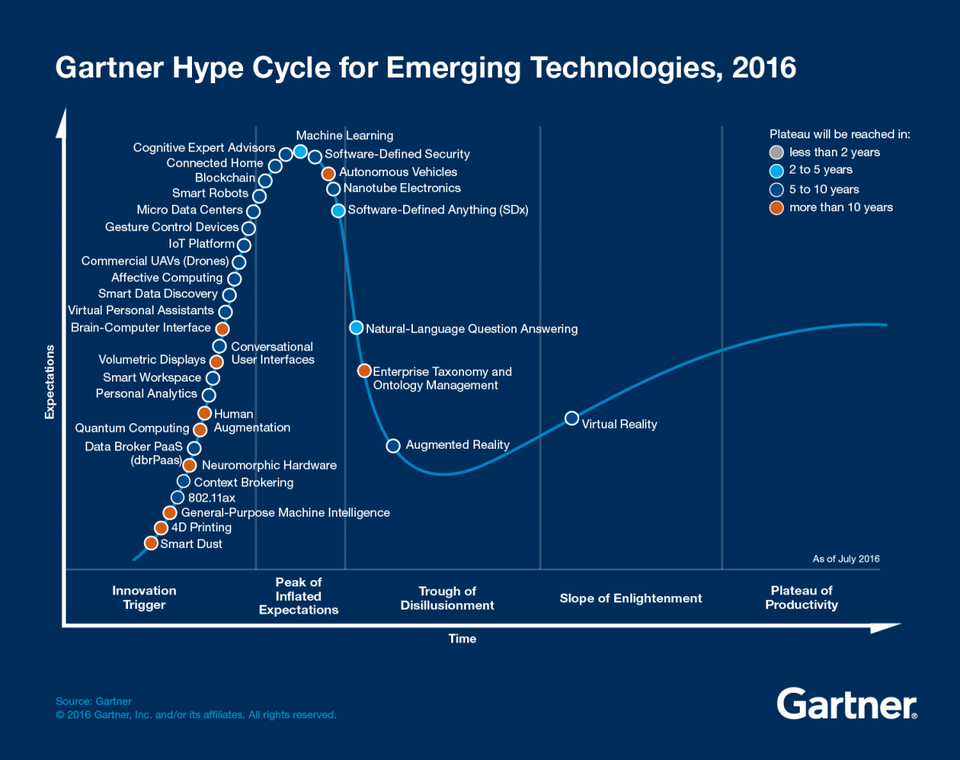
\includegraphics[width=0.9\linewidth]{img/Hype_Cycle_2016.jpg}
	\caption*{\protect\citeNP<Quelle:>[o.S.]{ghcet2016}}
	\label{fig:ghc2016}
\end{figure}

Demnach waren beispielsweise die Erwartungen und somit die Trendwahrnehmung für die Technologie \glqq Machine Learning\grqq~im Jahre 2016 am höchsten. Die Technologien links davon hatten eine geringere Reife, die rechts davon eine höhere. Insgesamt handelt es sich bei den Technologien allesamt um Trends des Jahres 2016 in der praktizierenden Wirtschaft.

Um den Trendverlauf der ausgewählten Technologien zu bestimmen, müssen weitere \glqq Hype Cyles\grqq~betrachtet werden. Das erstmalige Erscheinen in einer Publikation liefert einen Hinweis darauf, wann eine Technologie die Aufmerksamkeit der relevanten Gruppe von praktizierenden Wirtschaftlern erlangt hat. Die Verteilung der Vorkommnisse und Abwesenheiten der Technologien in den jeweiligen Ausgaben ermöglicht Rückschlüsse über den Zeitraum und Verlauf der Trendwahrnehmung.

Zur Ermittlung des erstmaligen Erscheinens werden solange vergangene \glqq Hype Cycles\grqq~betrachtet, bis die jeweils gesuchte Technologie in einer vorhergehenden Ausgabe fehlt. Für die meisten Technologien ist damit das Jahr der ersten Ausgabe ermittelt. Ist die Prognose der Dauer bis zum Erreichen des \glqq Plateaus\grqq~ mit größer als fünf Jahren angegeben, sind weitere Vorgänger zu betrachten, da eine Technologie in der Zeit vorübergehend unter die Trendschwelle fallen kann.

Für die Ermittlung des Trendverlaufs wird zusätzlich die aktuelle Ausgabe hinzugenommen.

Dabei sind folgende Parameter für die Auswertung festzuhalten:

\begin{enumerate}
	\item Name der Technologie
	\item Jahr der Ersterscheinung
	\item Jahr aller Erscheinungen mit Zuordnung zur jeweiligen Phase
\end{enumerate}

\subsubsection{Literaturdatenbanken}
Demgegenüber wird die Datenbasis der akademischen Forschung aus Abfragen in relevanten Literaturdatenbanken erhoben. Aufgrund ihrer hohen Abdeckung wissenschaftlich, technologischer Publikationen werden folgende Datenbanken durchsucht:
\begin{itemize}
	\item Web of Science Core Collection: \url{http://apps.webofknowledge.com}
	\item IEEE Xplore Digital Library: \url{https://ieeexplore.ieee.org}
	\item The ACM Guide to Computing Literature: \url{https://dl.acm.org}
\end{itemize}

Diese enthalten neben den in Abschnitt \ref{sec:acad_pub} genannten Fachzeitschriften und Tagungsbänden weitere Formen von Veröffentlichungen, wie beispielsweise Bücher oder Standards. Daher ist die Suche ausschließlich darauf einzugrenzen.

Alle Datenbanken sind im erweiterten Suchmodus mit vergleichbarer Funktionalität zur Vergabe von Suchkriterien ausgestattet. Diese sind gezielt einzusetzen, damit das Suchergebnis einerseits möglichst vollständig ist und andererseits keine \glqq False Positives\grqq~liefert. Deshalb beschränkt sich die Suche der Technologien auf die Metadaten Titel, Stichwörter und Abstract einer Publikation.



Die zuvor ermittelten Technologien aus Abschnitt \ref{sec:ghcet} werden zunächst unverändert in die Suchmaschine eingegeben, um eine Übersicht der Datenlage zu erhalten. Anschließend werden die Suchkriterien verfeinert

Über die Web-Oberfläche aller drei Datenbanken sind komplexe Abfragen sowie das Exportieren der Ergebnisse möglich. Lediglich in Syntax von Suchalgorithmen und Funktionsumfang des Exports unterscheiden sie sich teilweise von einander.

Die Anforderung an die 

Dabei ist zu berücksichtigen, dass Technologiebegriffe aus dem \glqq Hype Cycle\grqq~nicht unbedingt die Benennung in der akademischen Forschung widerspiegeln müssen.

\subsection{Operationalisierung der Daten}


Verstehen der Technologien
Synonyme finden
unterschiedliche Begrifflichkeiten feststellen
Kurve über die Zeit in Abhängigkeit zu Erwartungen

\subsection{Methodik der Analyse}